Nesta seção explicamos o processo da realização do trabalho, desde o desenho do projeto no papel e ideias iniciais até a criação dos ambientes físicos de demonstração, interface de criação de cenários (Physimulation) e finalmente as integrações com exercícios-programas.

\subsection{Estudo inicial}
Após nosso orientador nos apresentar as discussões e ideias do Grupo de Apoio ao BCC (seção \ref{introducao} e \ref{apendice}), decidimos planejar nosso trabalho de formatura levando em conta esta preocupação com os alunos do BCC. Inicialmente, nosso foco seria nas disciplinas de física (FAP-126) e estatística (MAE-121). \\

Partimos para a leitura de artigos e páginas da internet que tivessem relação com esta ideia. A seguir listamos algumas das referências mais interessantes neste processo:
\begin{itemize}
	\item \textit{An Introduction to Computer Simulation Methods: Applications to Physical Systems}, Gould, Tobochnik
	\item \textit{Evaluation of real-time physics simulation systems}, Boeing e Bräunl
	\item \textit{Esquema de detecção e resposta a colisões para animação física simplificada}, Temistocles, Atencio
	\item Box2D, (TODO site e explicação)
	\item Hotruby, (TODO site e explicação)
\end{itemize}

Percebemos que muitos estudos já havia sido feito na área de simulações e animações físicas, motivados principalmente pela criação de jogos para computador, \textit{video-games} e celulares. Neste último campo, com a recente expansão do uso de \textit{smartphones}, havia um número considerável de bibliotecas voltadas para reprodução de ambientes físicos. Durante esta fase pesquisa, o projeto começava a tomar mais forma e descartamos a possibilidade de trabalhar com a disciplina de estatística. A partir deste momento, concentraríamos esforços apenas em física. \\

Pesquisamos então as bibliotecas \textit{open-source} disponíveis e adequadas ao nosso objetivo de integração com a disciplina do IME.
Como já havíamos decidido trabalhar com a linguagem Ruby (seção \ref{plataforma}), procuramos por \textit{frameworks} nesta linguagem. Nesta fase de pesquisa, as bibliotecas que selecionamos para nosso trabalho foram o Chipmunk e Gosu (seção \ref{plataforma}). 

Além dos \textit{frameworks} vistos na seção anterior, outras bibliotecas foram consideradas para o projeto. Por exemplo...\\
Porém...\\
Então...

\begin{figure}[H]
	\centering
	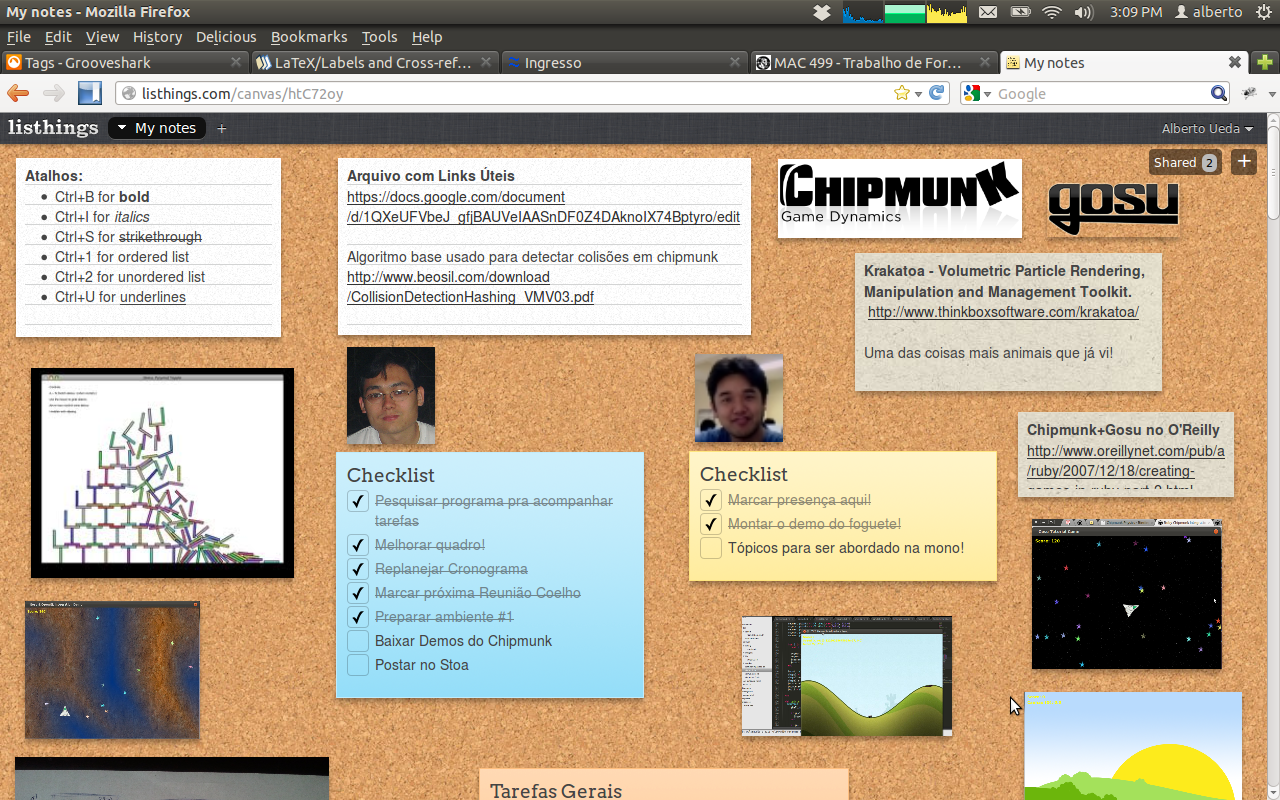
\includegraphics[scale=0.3]{images/listhings.png}
	\caption{Listhings - Aplicativo do Google Chrome para organização de tarefas }
\end{figure}

\begin{figure}[H]
	\centering
	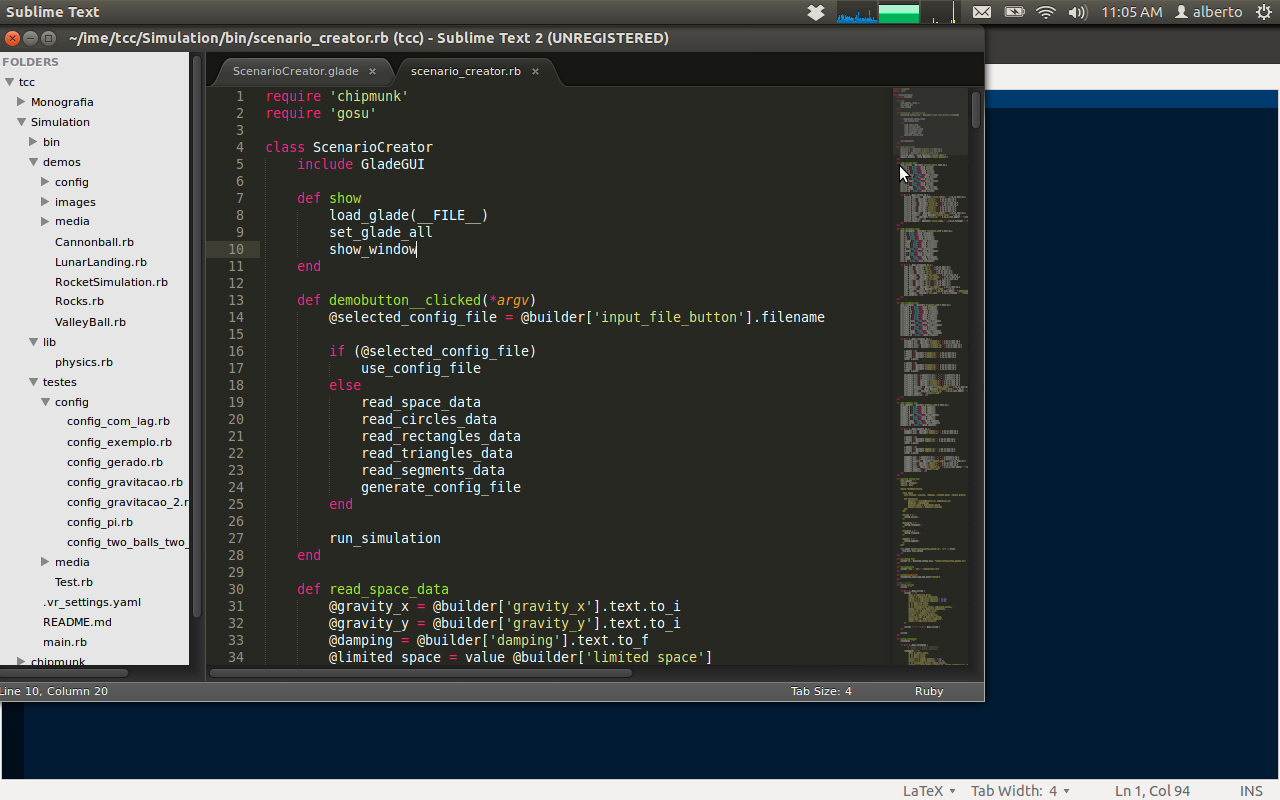
\includegraphics[scale=0.3]{images/sublime-text-2.png}
	\caption{Sublime Text 2 - Editor de Texto feito em Python}
\end{figure}

\subsection{Ambientes de demonstração}
Após definida a linguagem e as ferramentas que utilizaríamos no trabalho, partimos...

\begin{figure}[H]
	\centering
	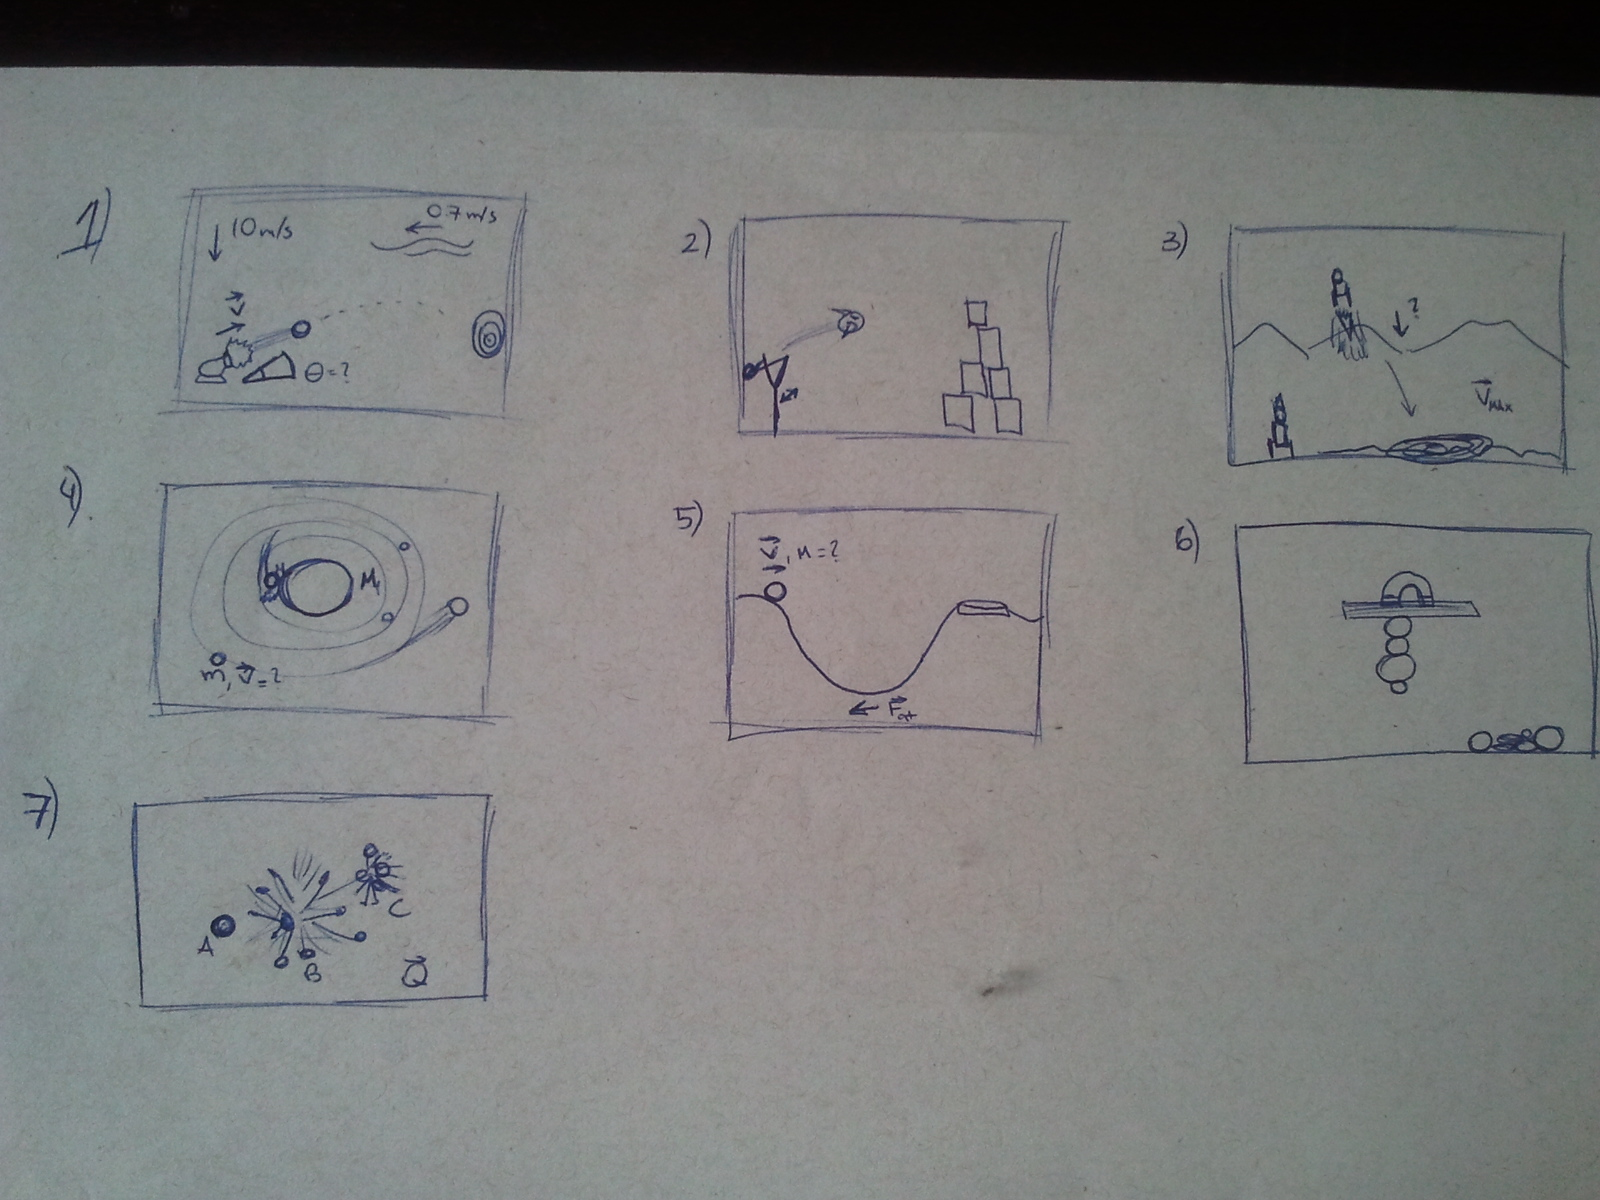
\includegraphics[scale=0.2]{images/tcc-demos.jpg}
	\caption{Primeiros rascunhos das demonstrações}
\end{figure}

\subsection{Criador de Cenários}
Com um conhecimento mais profundo das bibliotecas após a implementação dos ambientes de demonstração, começamos a montar a interface de criação de cenários físicos. Como já tínhamos esta ideia em mente desde o início do projeto, centralizamos boa parte do código que era importante em classes que facilitariam a criação de simulações genéricas. Esta estratégia nos facilitou bastante o trabalho desta etapa.\\

Encontramos o glade...

\begin{figure}[H]
	\centering
	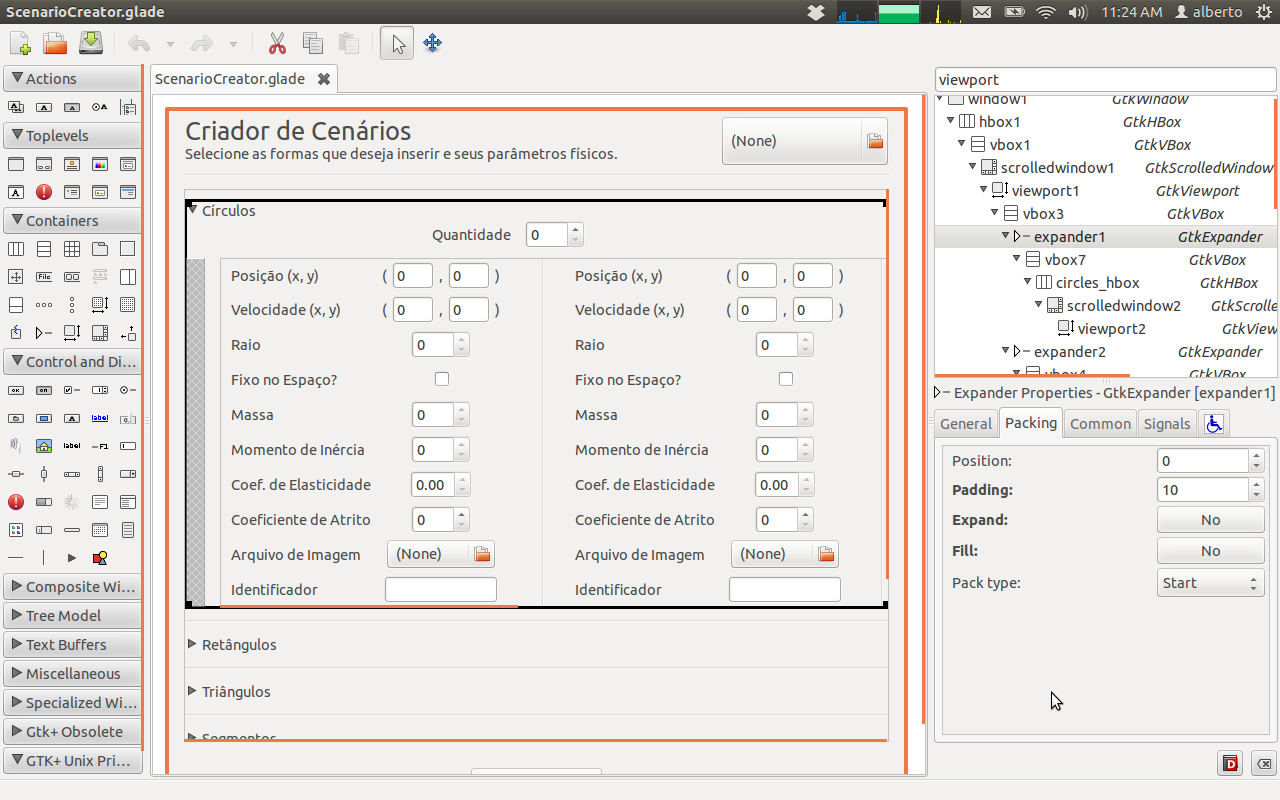
\includegraphics[scale=0.3]{images/glade.png}
	\caption{Gnome Glade}
\end{figure}

Discutímos durante as reuniões com o orientador e o João Kerr como seria a interface, as propriedades físicas que poderiam ou não poderiam ser alteradas...

Falar da questão do momento de inércia...

\begin{figure}[H]
	\centering
	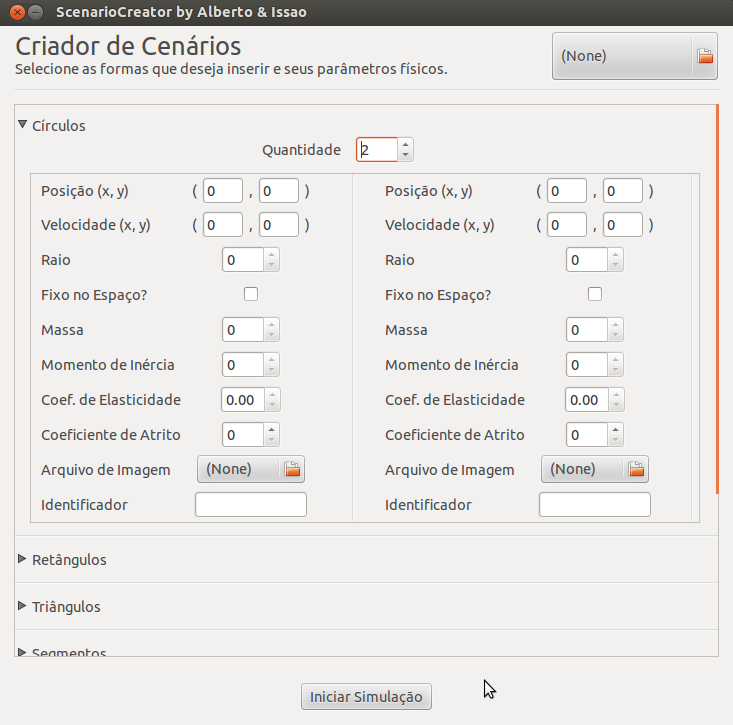
\includegraphics[scale=0.5]{images/physimulation.png}
	\caption{Interface ao final das discussões}
\end{figure}

